\documentclass{beamer} 
\usepackage{amsmath,amsthm}
\usepackage{graphicx,microtype,parskip}
\usepackage{caption,subcaption,multirow}
\usepackage{attrib}
\usepackage{array}

\frenchspacing

\usetheme{default}
\usecolortheme{whale}

\setbeamertemplate{navigation symbols}{}

\setbeamercolor{title}{fg=blue,bg=white}

\setbeamercolor{block title}{fg=white,bg=gray}
\setbeamercolor{block body}{fg=black,bg=lightgray}

\setbeamercolor{block title alerted}{fg=white,bg=darkgray}
\setbeamercolor{block body alerted}{fg=black,bg=lightgray}


\title{How predictable is extinction?} 
\subtitle{Forecasting species survival at million-year timescales}
\author{Peter D Smits, Seth Finnegan}
\institute{Department of Integrative Biology, University of California -- Berkeley}
\date{}


\begin{document}


\begin{frame}
  \maketitle
\end{frame}


\begin{frame}
  \frametitle{Foundational assertion of conservation paleobiology }

  \begin{center}
    \begin{LARGE}
      By studying the \alert{past}, \\we can better predict the \alert{future}.
    \end{LARGE}
  \end{center}

\end{frame}


\begin{frame}
  \frametitle{What are we predicting?}

  \begin{center}
    \begin{LARGE}
      Extinction is \alert{hard} to predict, but is \alert{important} to conservation decisions.
    \end{LARGE}
  \end{center}

\end{frame}


\begin{frame}
  \frametitle{Predicting extinction}

  \begin{itemize}[<+->]
    \item A taxon with a \alert{greater than average} global geographic range is likely to \alert{survive for longer} than a taxon with \alert{less than average} global geographic range.
    \item A taxon's global geographic range can change over time.
    \item What happens to extinction risk as a taxon changes geographic range? How is extinction risk impacted if that taxon's global geographic range has recently \alert{increased} or \alert{decreased}?
  \end{itemize}

\end{frame}


\begin{frame}
  \frametitle{Data being analyzed}

  \begin{columns}
    \begin{column}{0.5\textwidth}
      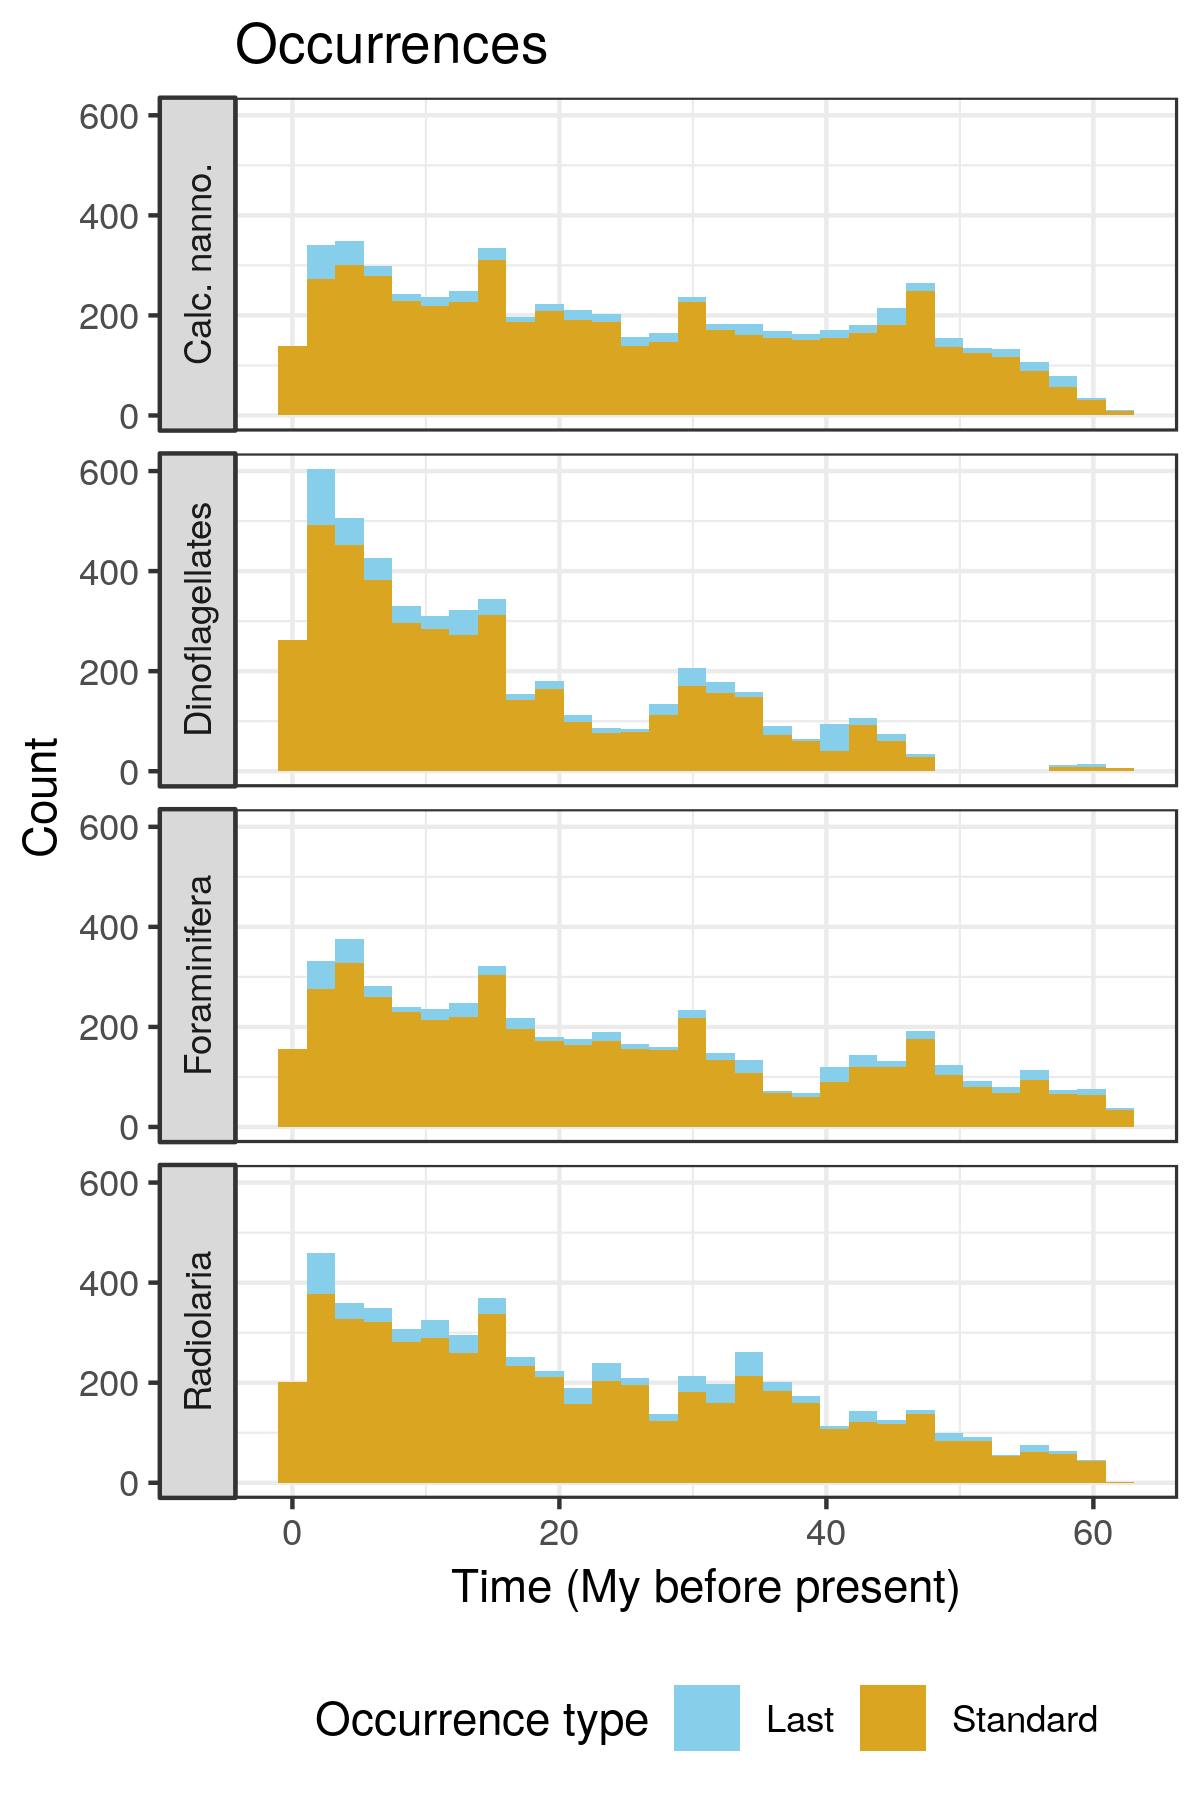
\includegraphics[width=\textwidth,height=0.8\textheight,keepaspectratio=true]{../results/figure/occ_time_label}
    \end{column}
    \begin{column}{0.5\textwidth}
      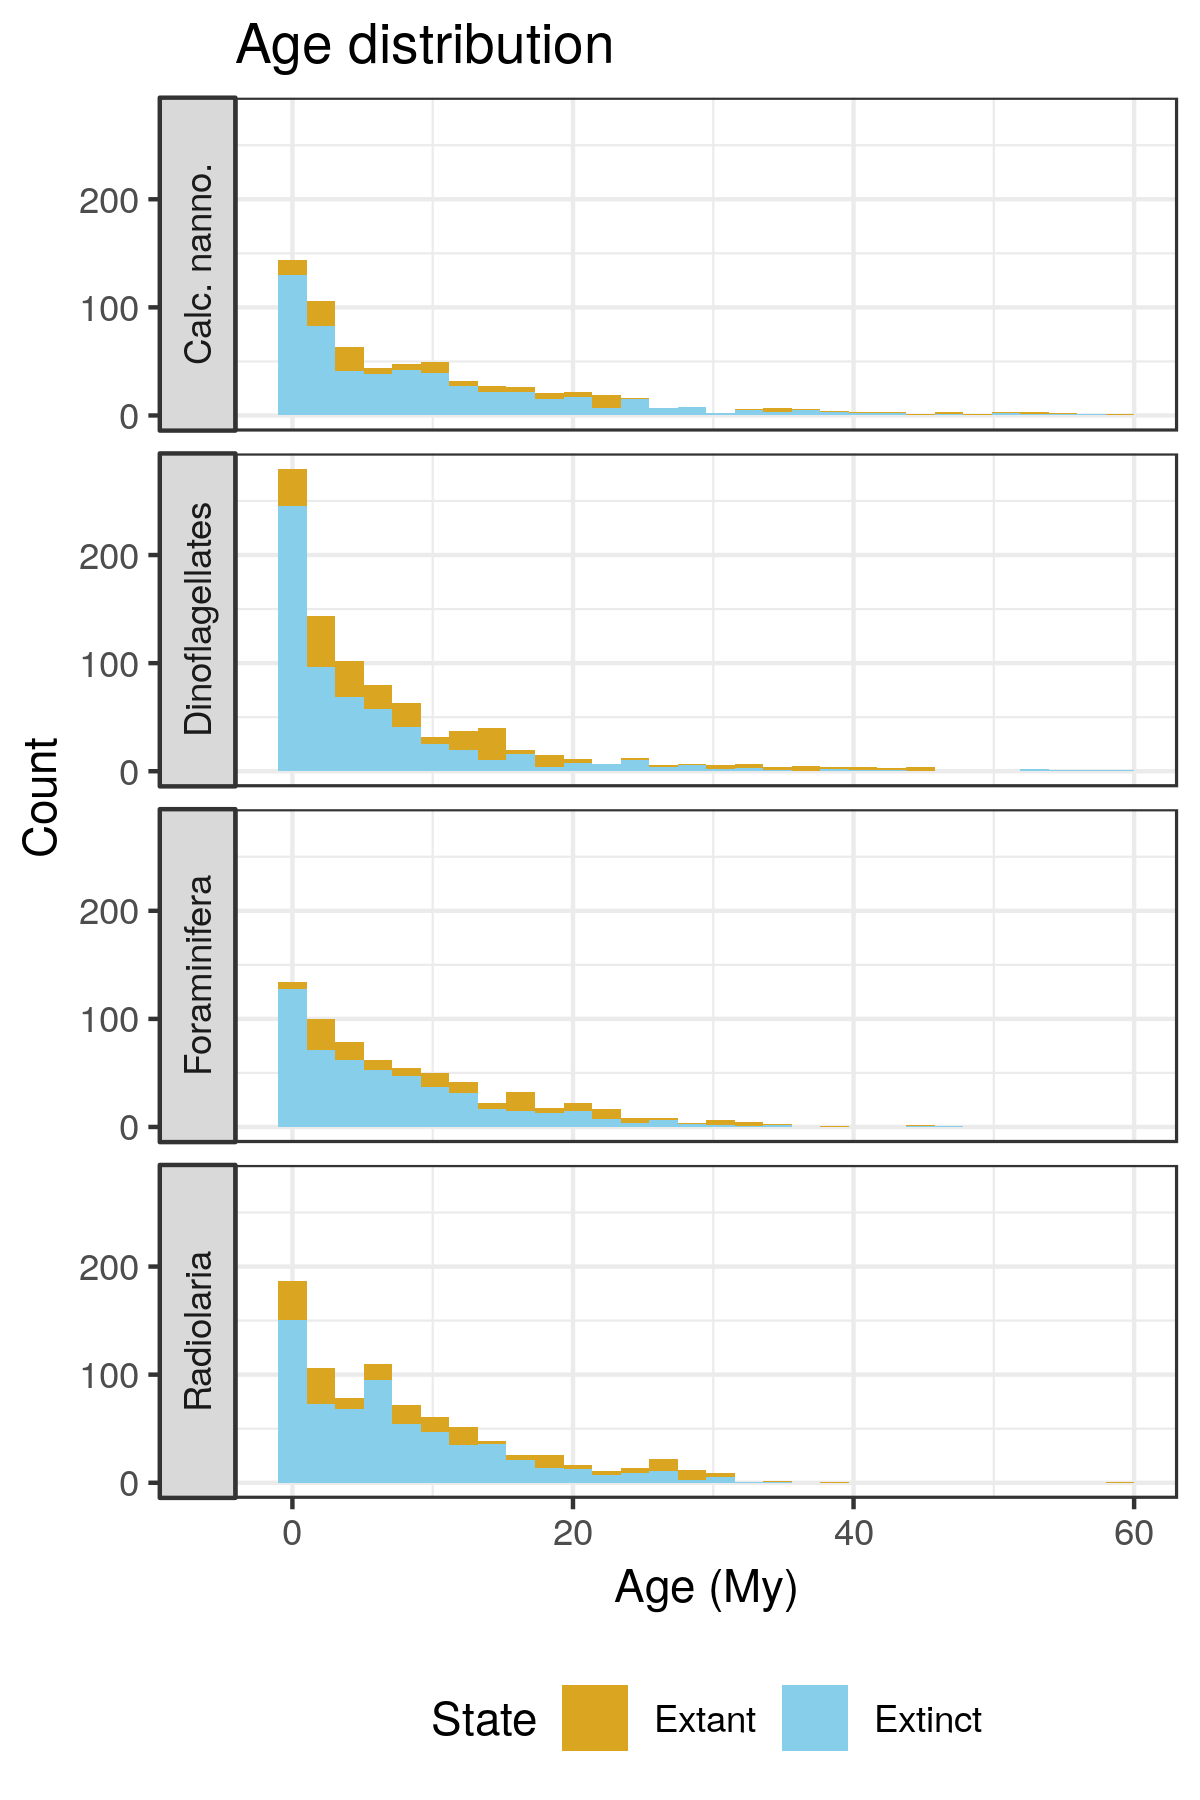
\includegraphics[width=\textwidth,height=0.8\textheight,keepaspectratio=true]{../results/figure/age_label}
    \end{column}
  \end{columns}

\end{frame}


\begin{frame}
  \frametitle{How we're analyzing the data}

  \begin{itemize}%[<+->]
    \item Encoding the past
      \begin{itemize}
        \item Change in geographic range between current observation and previous observation.
        \item Average global temperature at time of previous observation (Mg/Ca isotope).
        \item Age in millions of years at time of observation.
      \end{itemize}
    %\item \alert{Compare} models using WAIC/LOOIC.
    \item Explore model adequacy using posterior predictive distribution.
    \item Estimate out-of-sample predictive performance using \(k\)-fold cross-validation.
  \end{itemize}

\end{frame}


\begin{frame}
  \frametitle{A conceptual model for predicting extinction}
      
  \begin{center}
    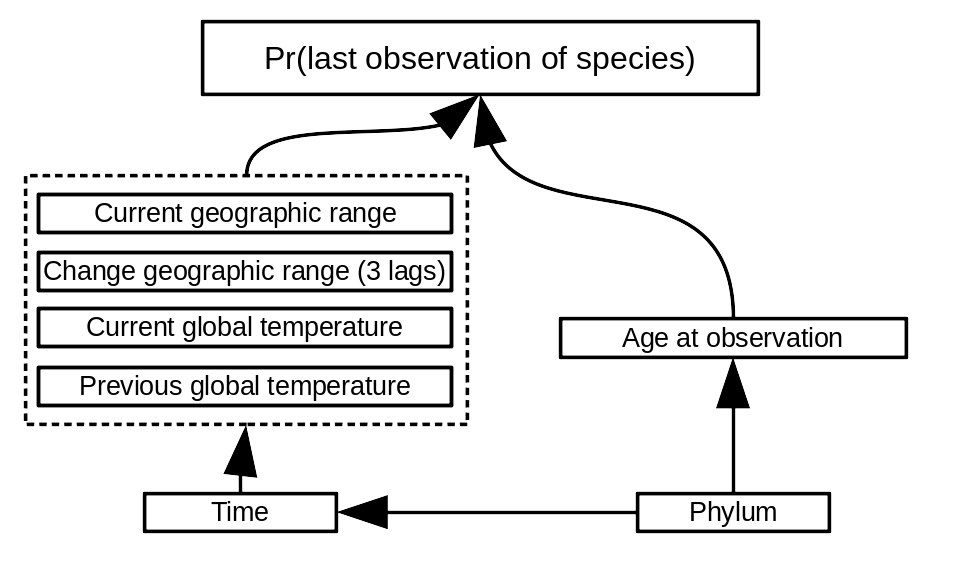
\includegraphics[width=\textwidth,height=\textheight,keepaspectratio=true]{figure/conceptual_diagram}
  \end{center}

\end{frame}


\begin{frame}
  \frametitle{Measuring performance: confusion matrix}

  \begin{center}
    \begin{tabular}[c]{ p{2cm} c | p{2cm} | p{2cm} |}
      \cline{3-4} 
      & & \multicolumn{2}{ c |}{Actual class} \\ \cline{3-4}
      & & 1 & 0 \\ \hline
      \multicolumn{1}{| c |}{\multirow{2}{*}{Predicted class}}
      & 1 & TRUE \newline POSITIVE & FALSE \newline POSITIVE \\ \cline{2-4}
      \multicolumn{1}{| c |}{} & 0 & FALSE \newline NEGATIVE & TRUE \newline NEGATIVE \\
      \hline
    \end{tabular}
  \end{center}

\end{frame}


\begin{frame}
  \frametitle{Measuring performance: Receiver Operating Characteristic}

  \begin{center}
    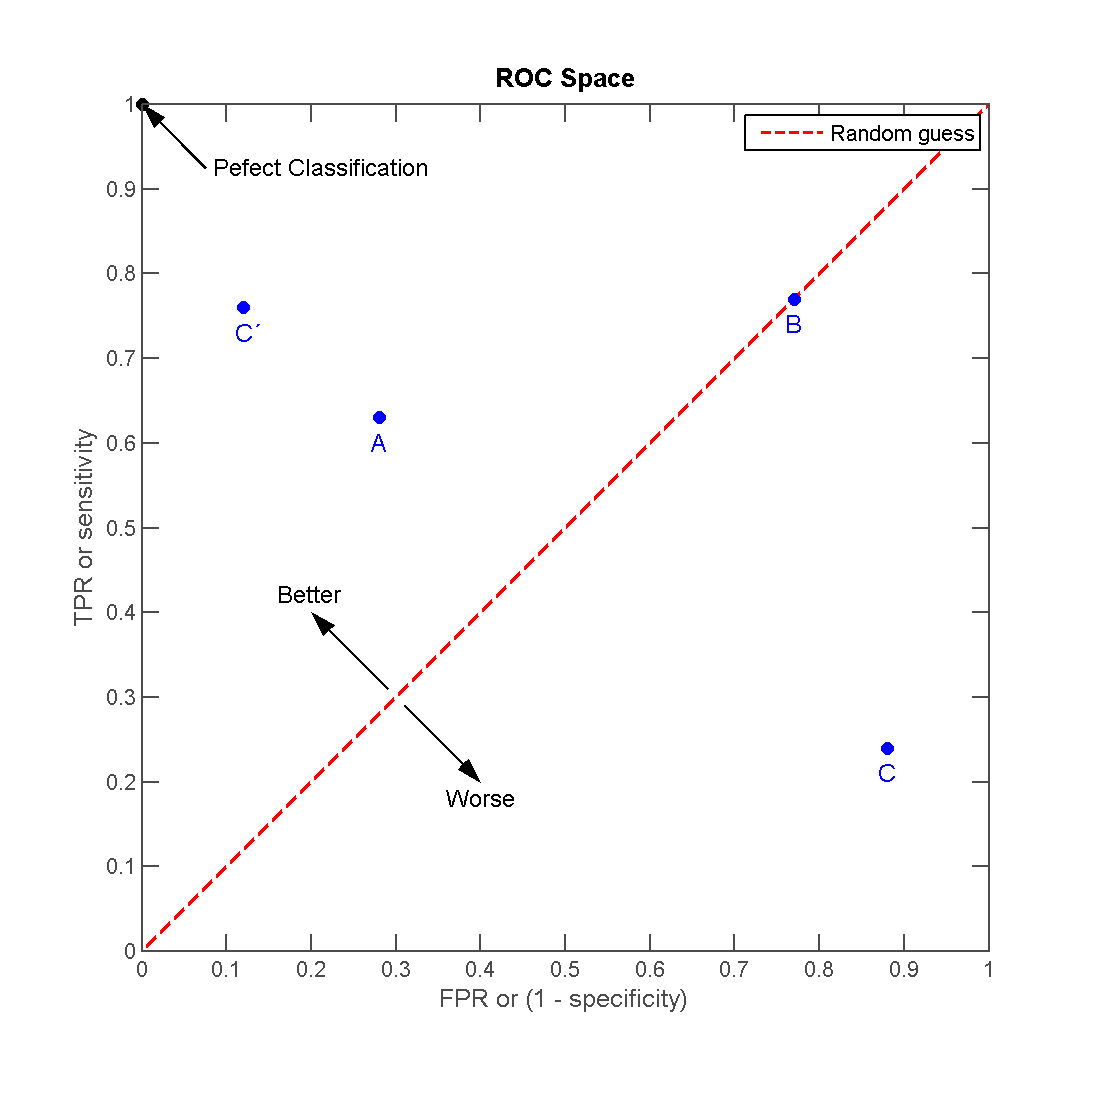
\includegraphics[width=\textwidth,height=0.8\textheight,keepaspectratio=true]{figure/wiki_ROC_space-2}
  \end{center}
  
  \attrib{\footnotesize{wikimedia}}

\end{frame}


\begin{frame}
  \frametitle{Measuring performance: Receiver Operating Characteristic}
  
  \begin{center}
    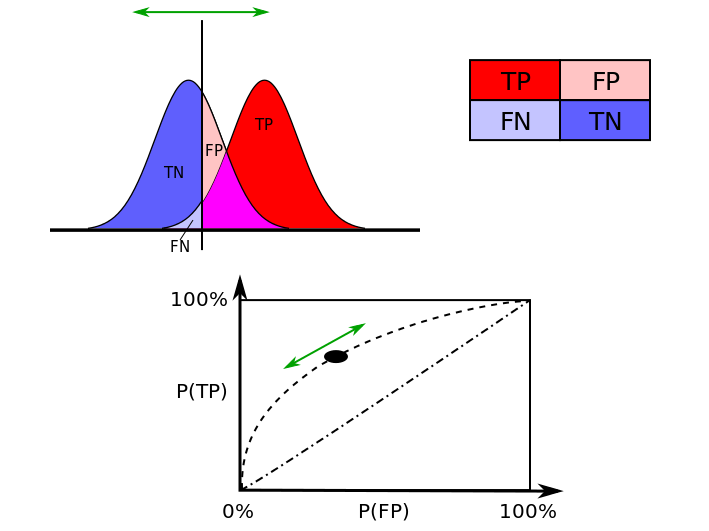
\includegraphics[width=\textwidth,height=0.75\textheight,keepaspectratio=true]{figure/wiki_709px-ROC_curves}
  \end{center}
  
  \attrib{\footnotesize{wikimedia}}
  
\end{frame}


\begin{frame}
  \frametitle{Measuring performance: \textit{k}-fold cross-validation}

  \begin{center}
    \includegraphics[width=\textwidth,height=0.8\textheight,keepaspectratio=true]{figure/ts_cv}
  \end{center}


  \attrib{\footnotesize{Ken Williams, https://goo.gl/qLcfL8}}
\end{frame}


% demonstrate as ROC curve
\begin{frame}
  \frametitle{In-sample predictive performance, full dataset}

  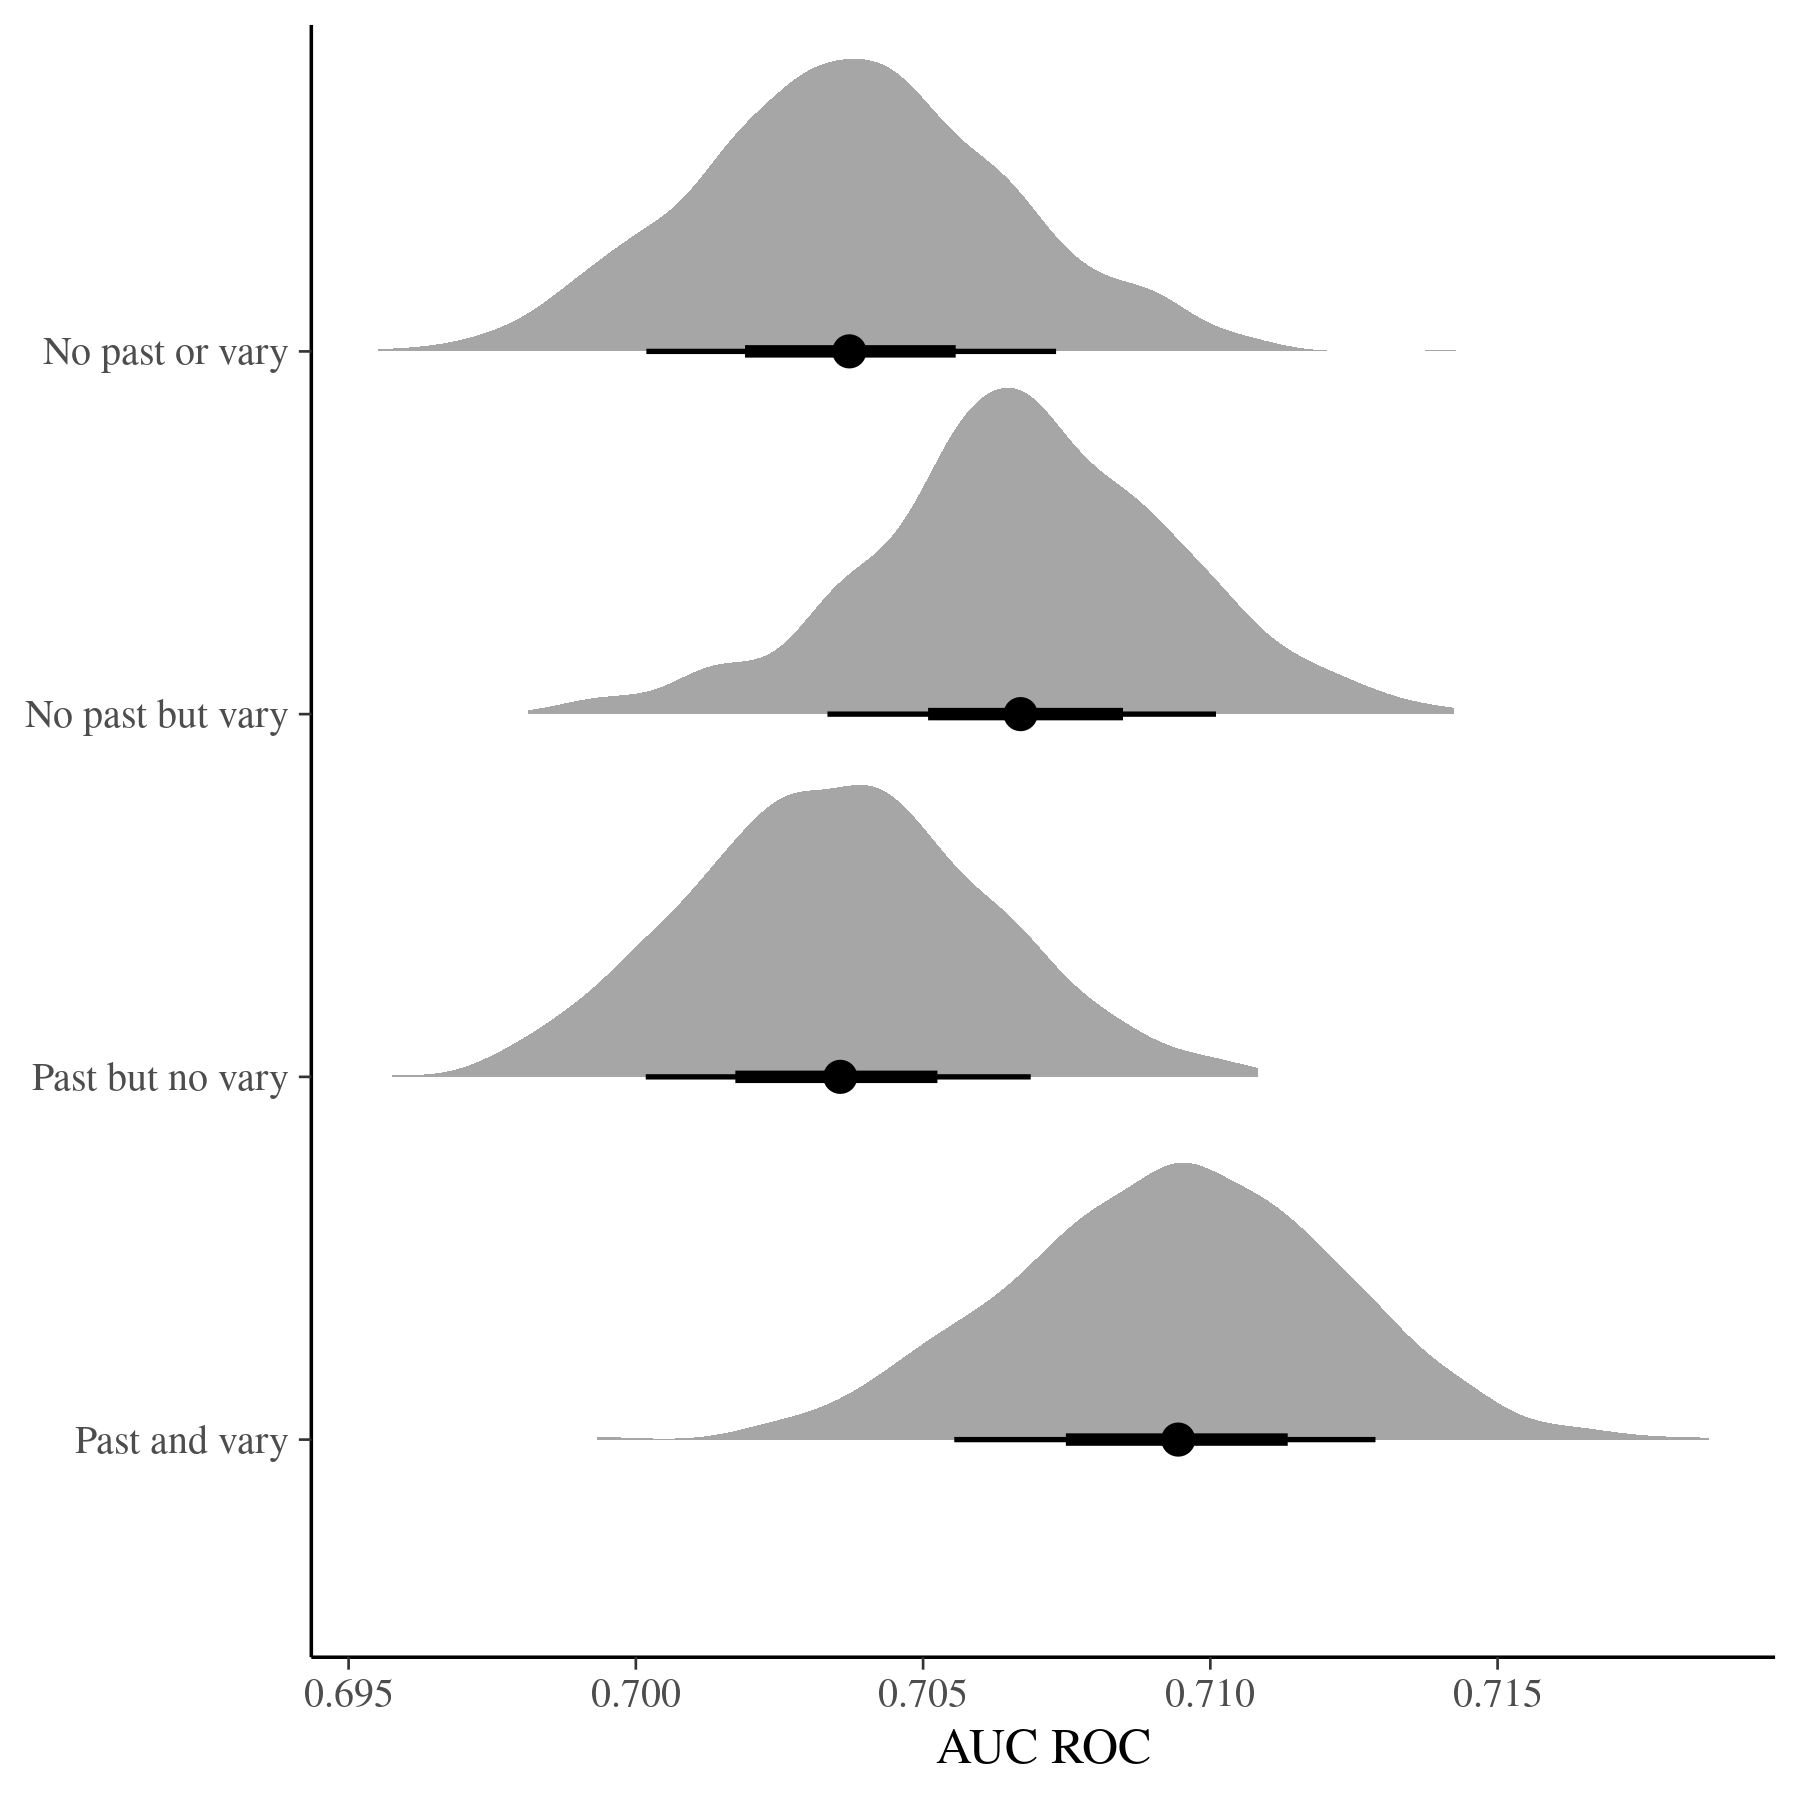
\includegraphics[width=\textwidth,height=0.8\textheight,keepaspectratio=true]{../results/figure/roc_hist}

\end{frame}


\begin{frame}
  \frametitle{In-sample predictive performance, by time}

  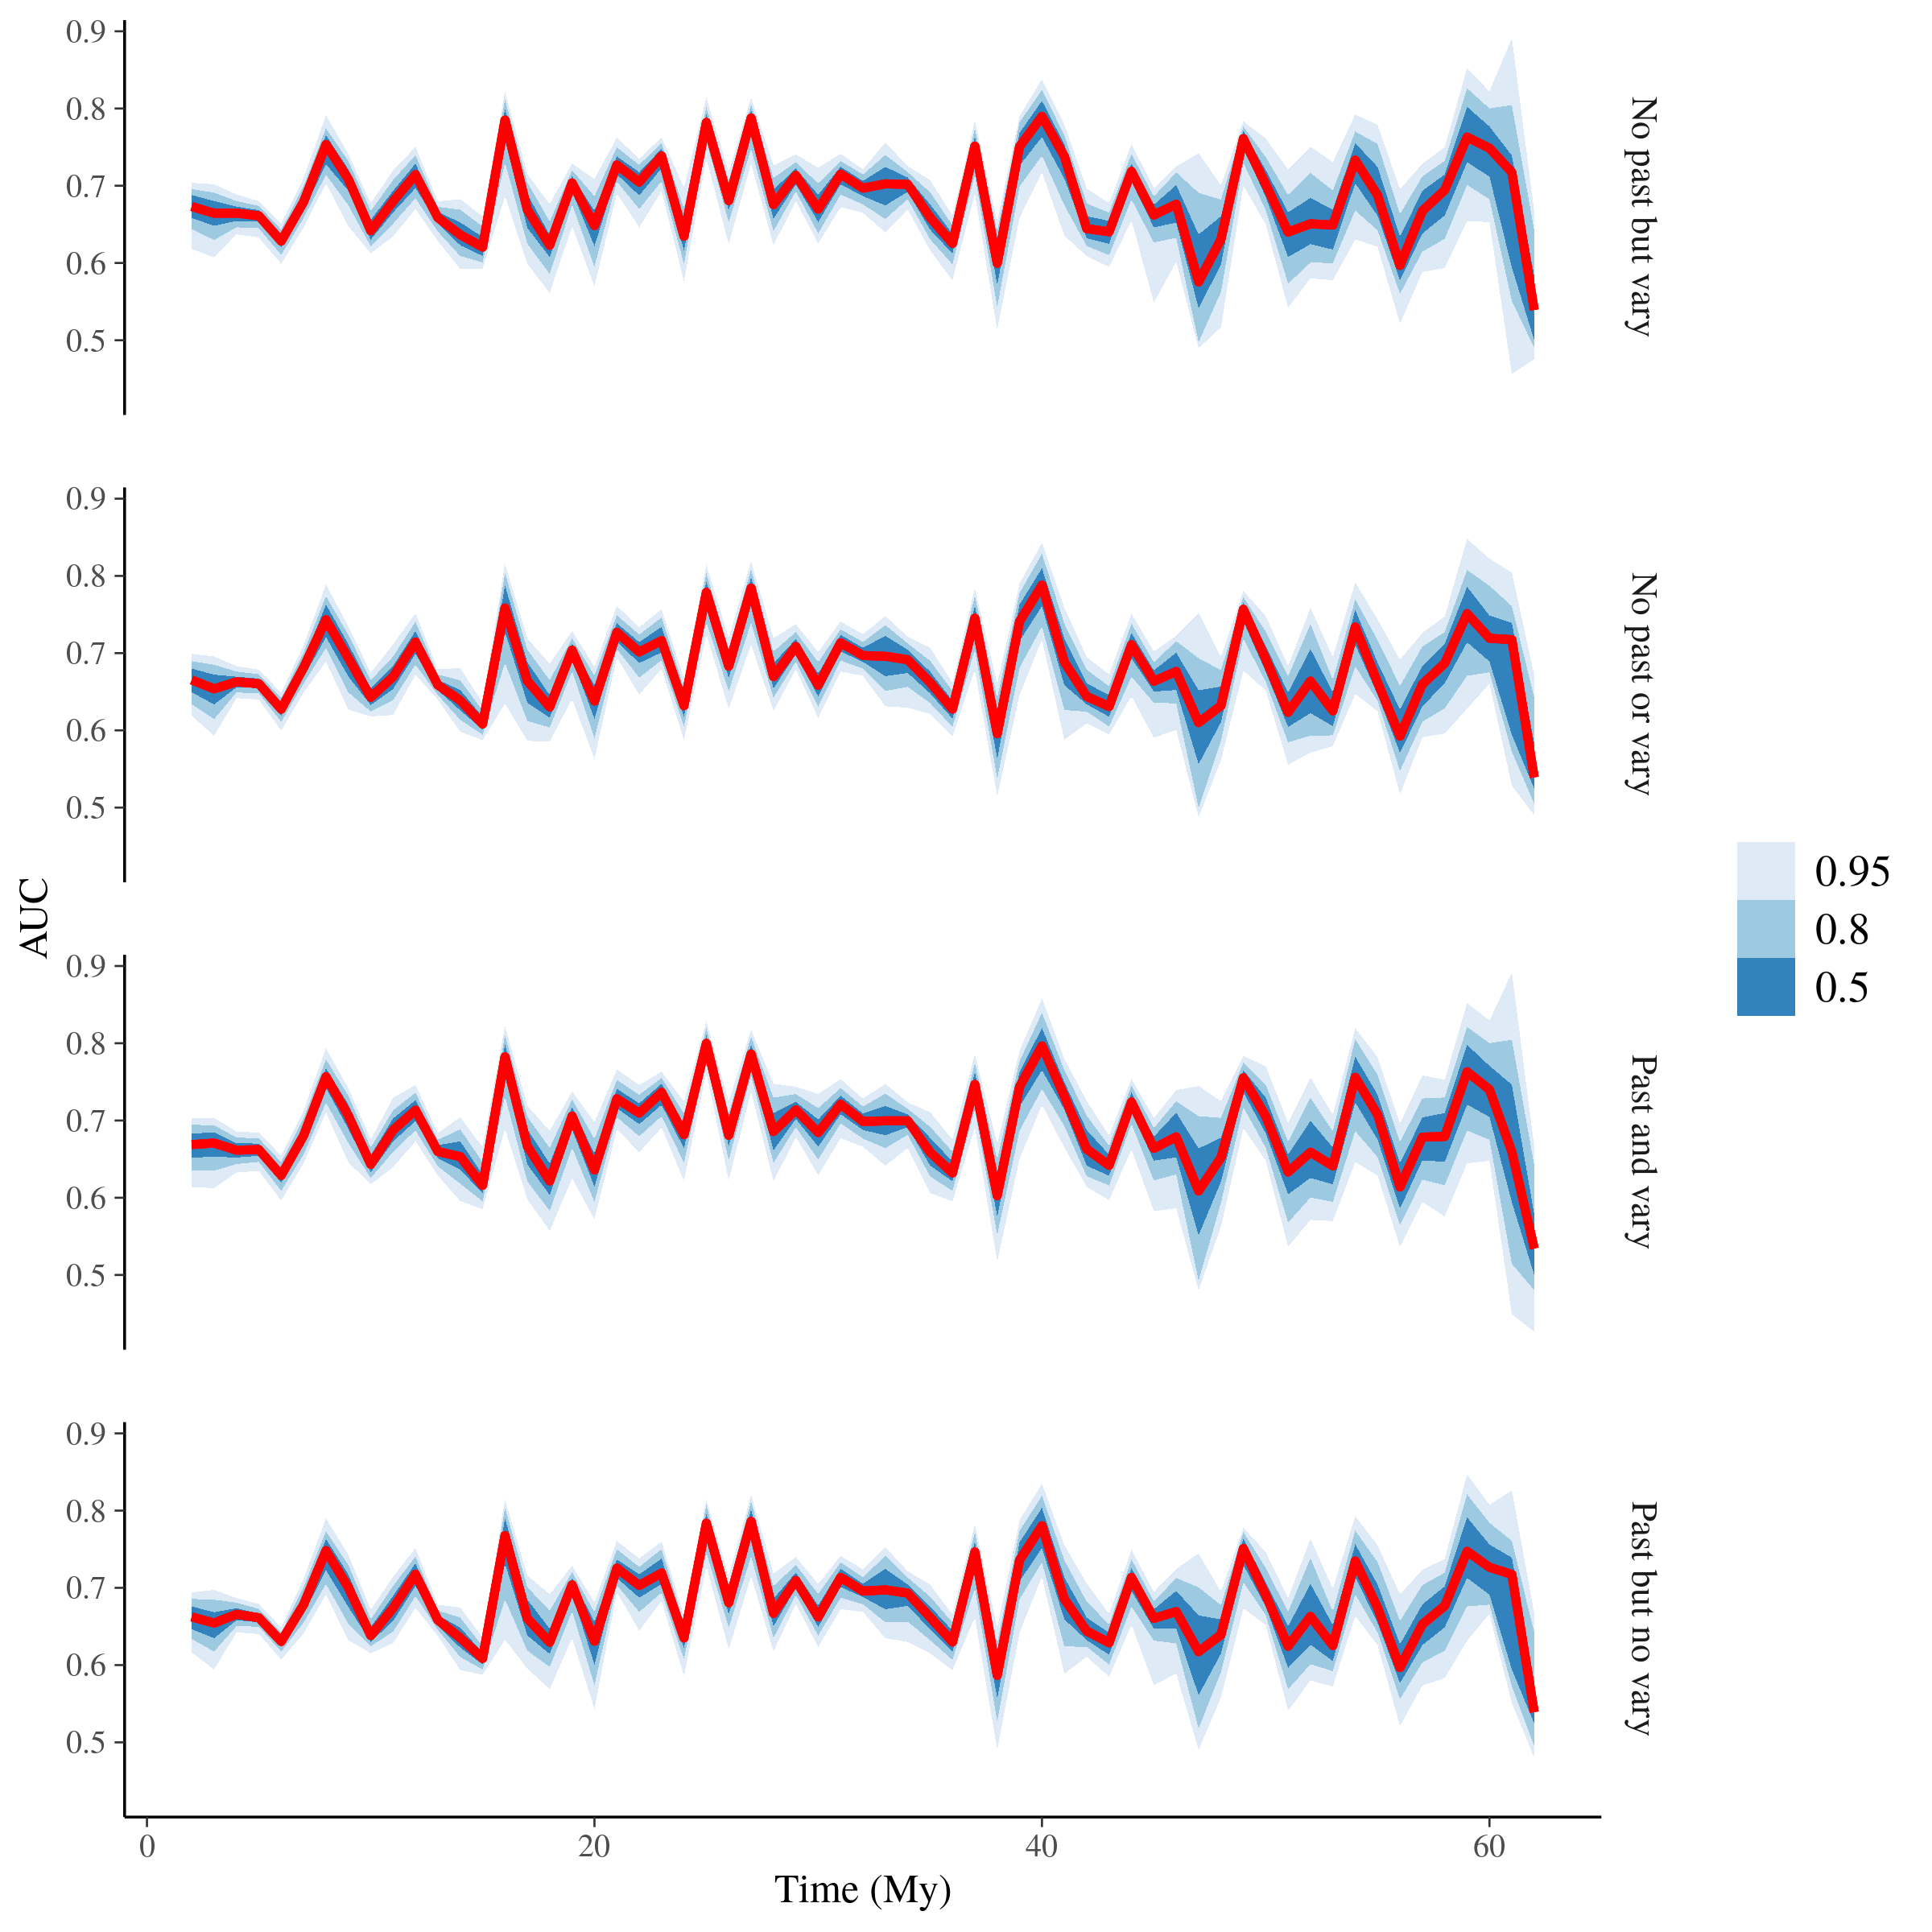
\includegraphics[width=\textwidth,height=0.8\textheight,keepaspectratio=true]{../results/figure/roc_ts}

\end{frame}


\begin{frame}
  \frametitle{Cross-validation results, full dataset}

  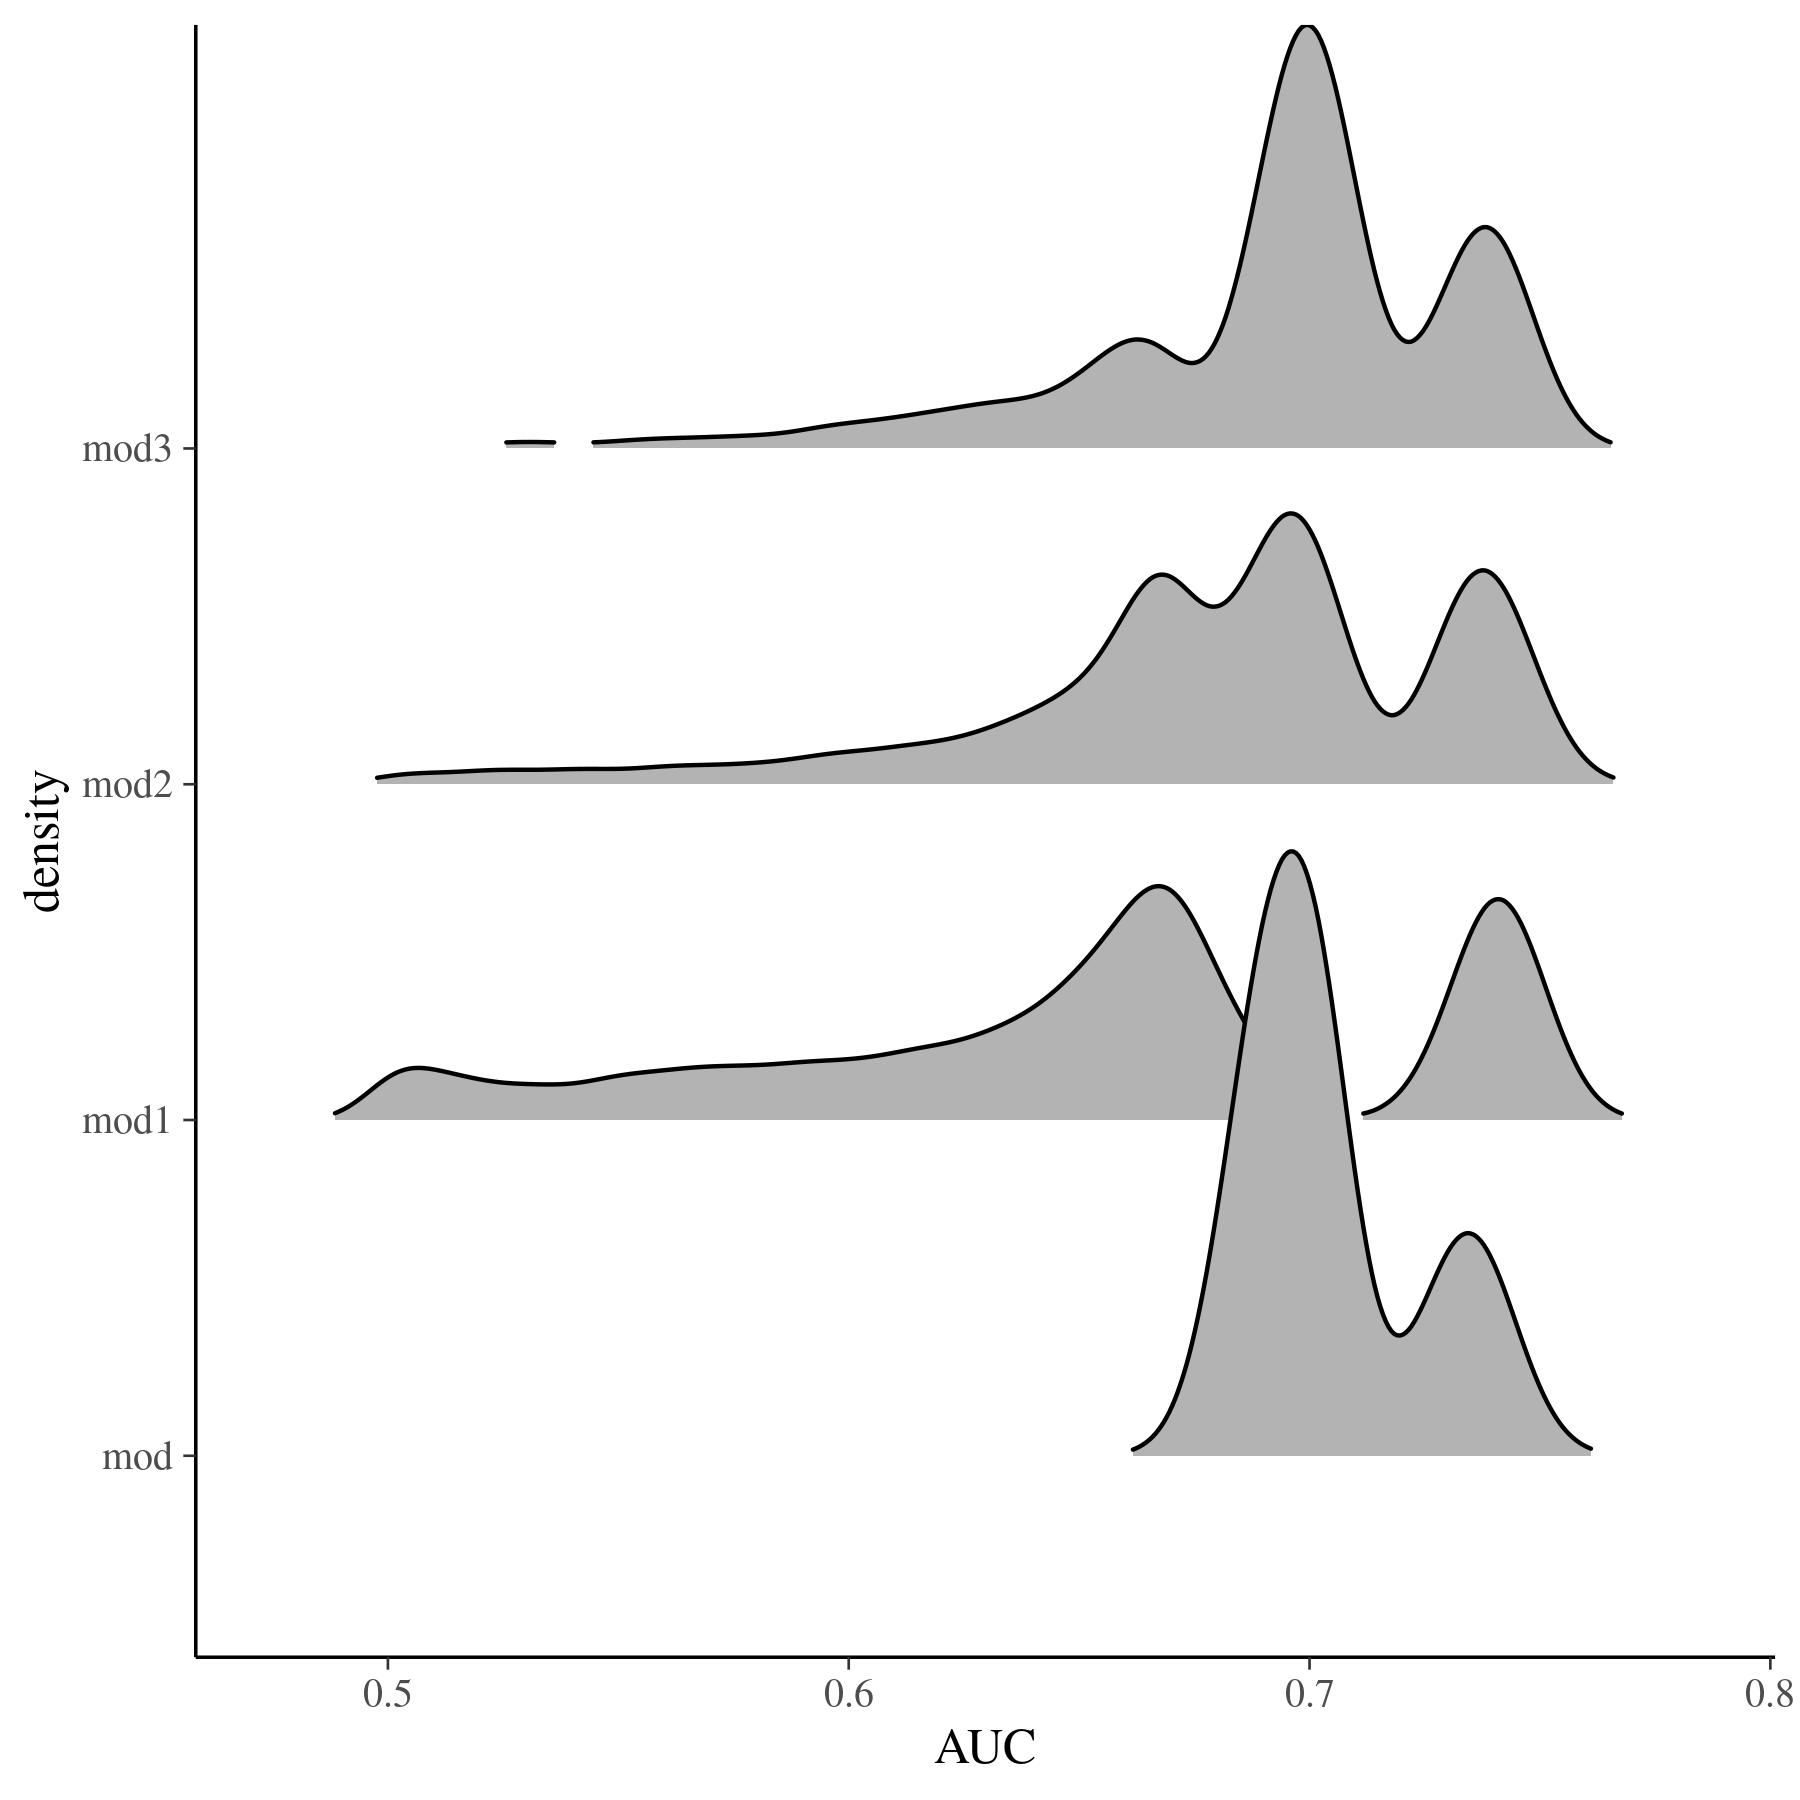
\includegraphics[width=\textwidth,height=0.8\textheight,keepaspectratio=true]{../results/figure/fold_auc}

\end{frame}


\begin{frame}
  \frametitle{Cross-validation results, by time}

  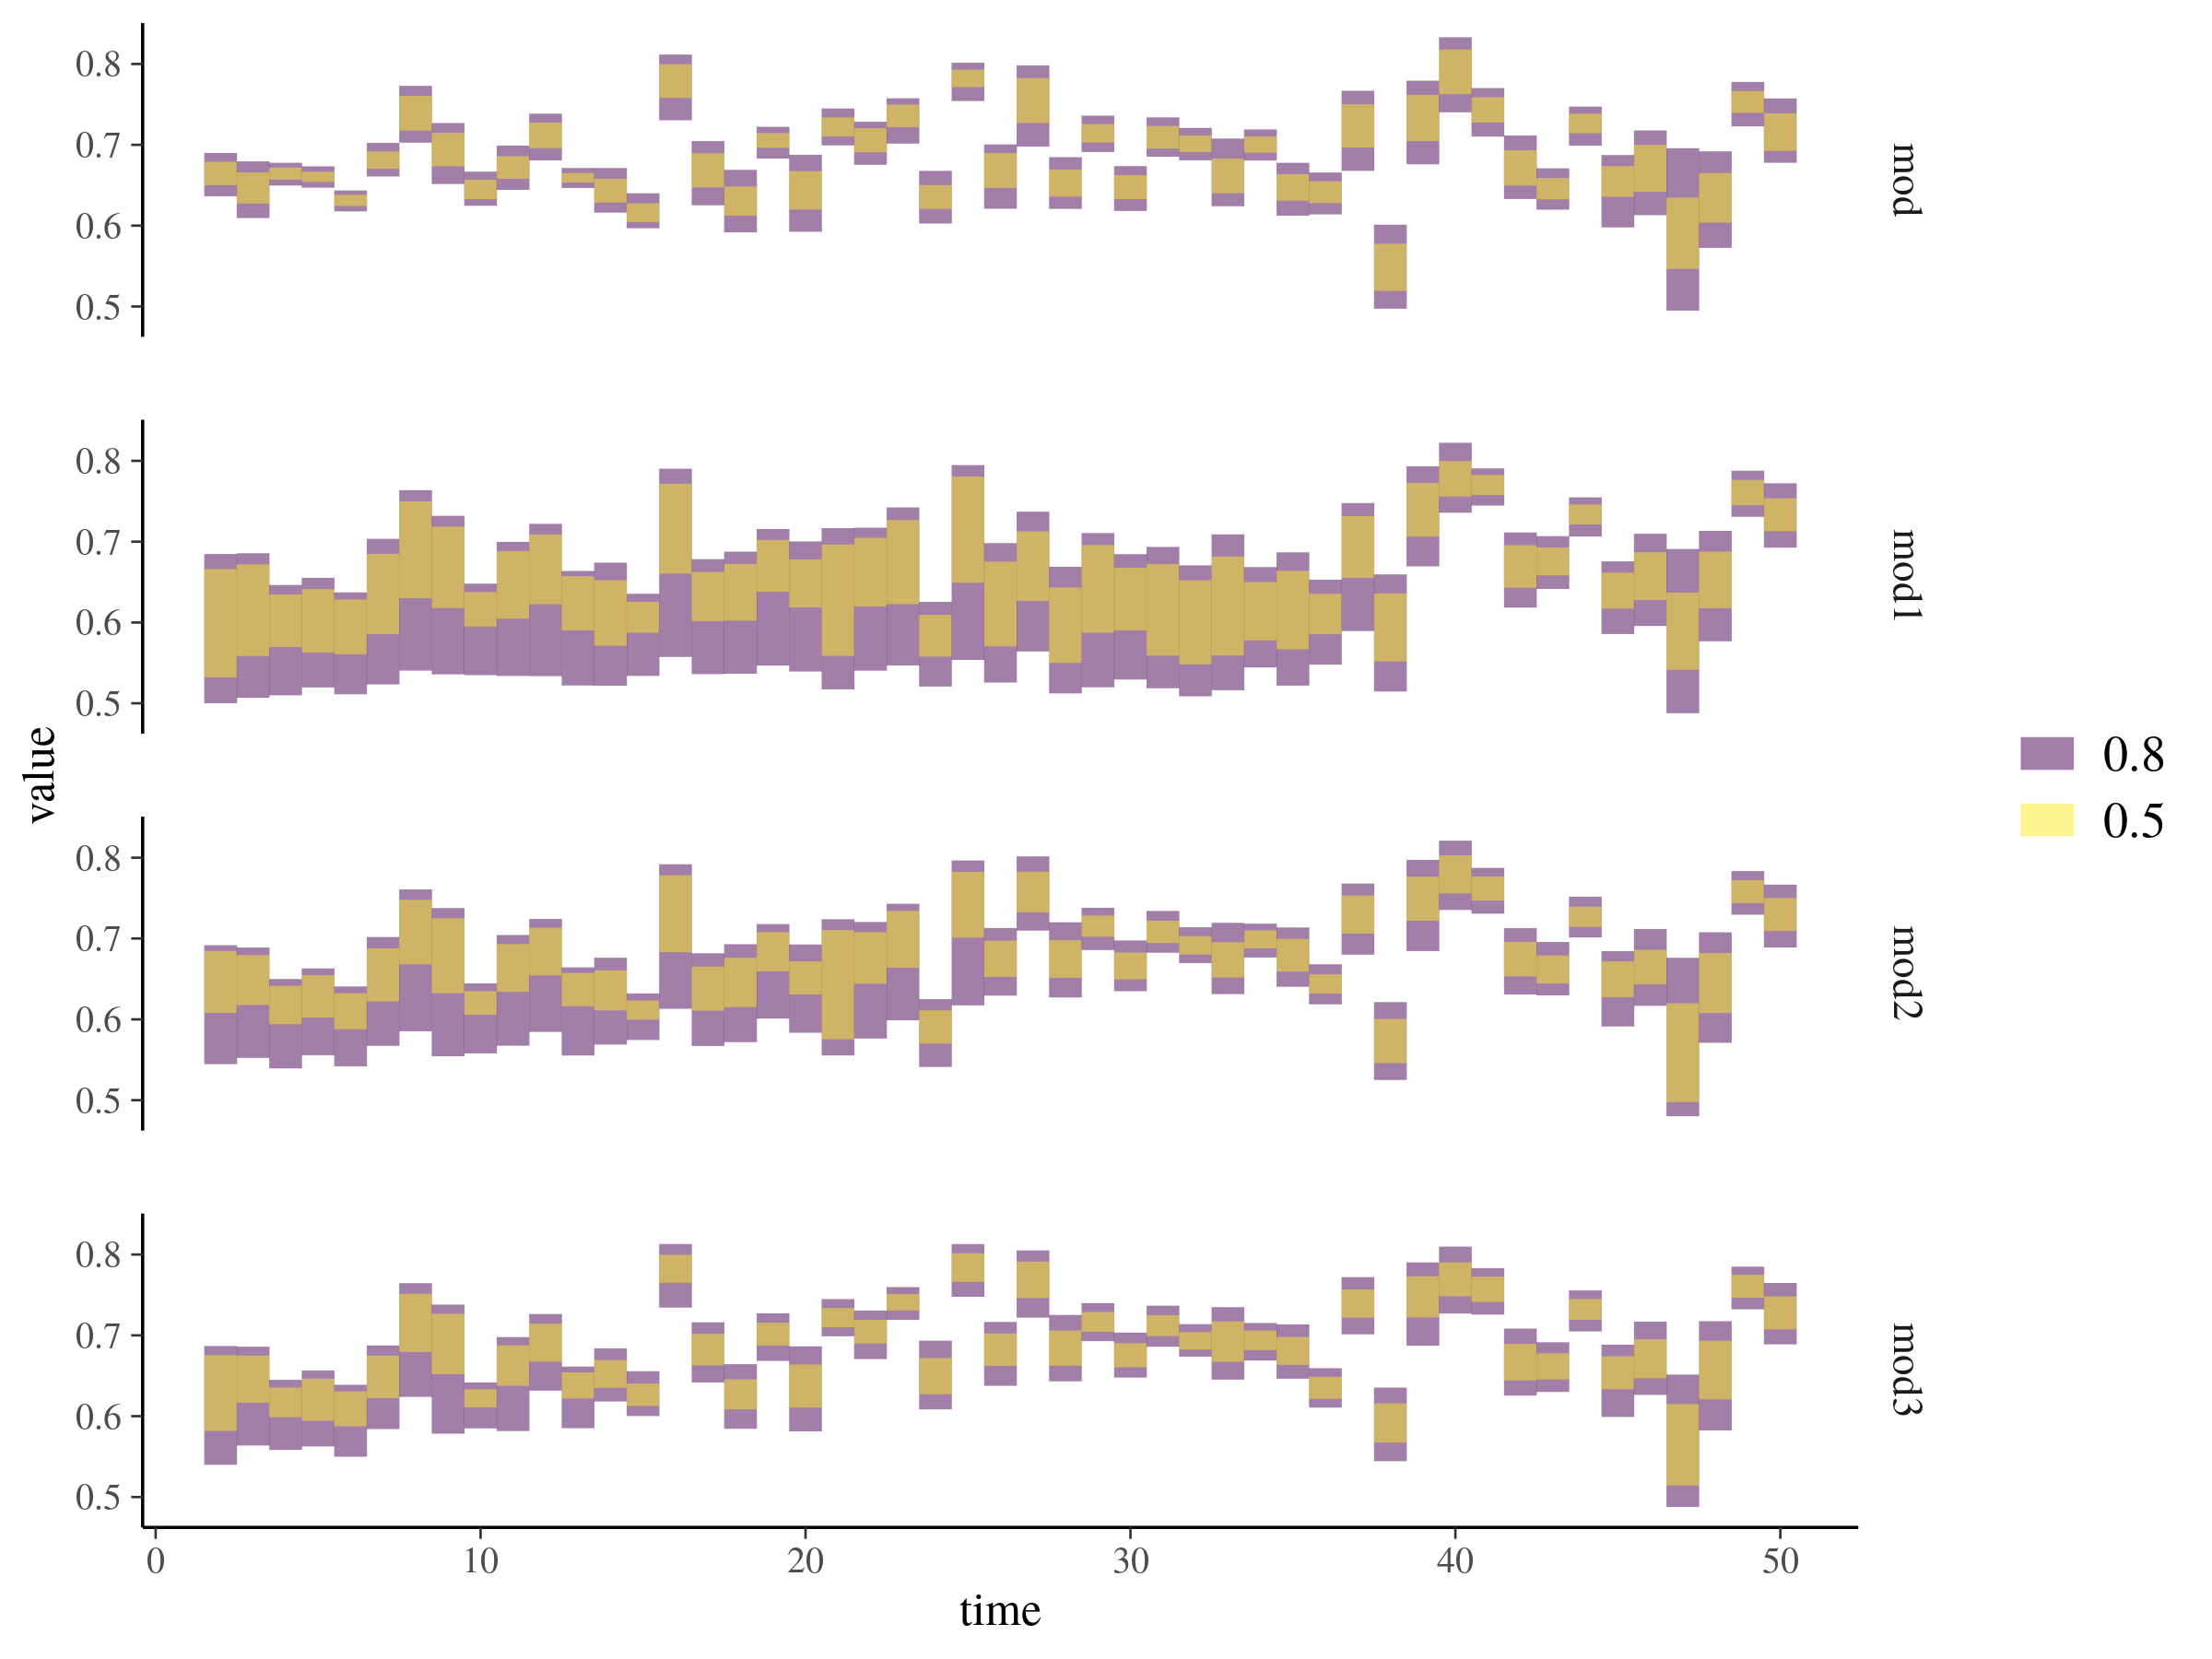
\includegraphics[width=\textwidth,height=0.8\textheight,keepaspectratio=true]{../results/figure/fold_auc_time}

\end{frame}


\begin{frame}
  \frametitle{Summary}

  \begin{itemize}
    \item \alert{The past matters\dots} 
      \begin{itemize}
        \item Our best supported model includes our historical covariates and allows all effects to vary over time.
      \end{itemize}
    \item \alert{But not that much\dots}
      \begin{itemize}
        \item None of our models are good at predicting extinction.
      \end{itemize}
    \item<2-> Mechanisms behind changes to geographic range operate at sub-million year scales. Perhaps their effects are weak/masked at million (or greater) year scales.
  \end{itemize}

\end{frame}


\begin{frame}
  \frametitle{Acknowledgements}

\end{frame}


\end{document}
